\documentclass[twoside,11pt,ShortChapTitles]{BYUTextbook}

\usepackage{soul}
\renewcommand{\vec}[1]{\ensuremath{\mathbf{#1}}}
\usepackage{siunitx}
\sisetup{round-mode = figures,
  round-precision = 3, scientific-notation=true}
  \usepackage{marginfix}

\usepackage{mathtools}

\usepackage{listings}
\usepackage{tabularray,varwidth}
\usepackage{color}

\definecolor{dkgreen}{rgb}{0,0.6,0}
\definecolor{gray}{rgb}{0.5,0.5,0.5}
\definecolor{mauve}{rgb}{0.58,0,0.82}

\lstset{frame=tb,
  language=Python,
  aboveskip=3mm,
  belowskip=3mm,
  showstringspaces=false,
  columns=flexible,
  basicstyle={\small\ttfamily},
  numbers=none,
  numberstyle=\tiny\color{gray},
  keywordstyle=\color{blue},
  commentstyle=\color{dkgreen},
  stringstyle=\color{mauve},
  breaklines=true,
  breakatwhitespace=true,
  tabsize=3, upquote=true}

\lstMakeShortInline[columns=fixed]|
\setcounter{chapter}{6}

\begin{document}



\chapter[Numerical modeling I]{Numerical modeling of Projectile motion}
\setcounter{page}{1}
\section*{Python You Should Know for This Chapter}
\begin{itemize}
\item How to construct a \code{for} loop.
\end{itemize}
Recommended reading: Introduction to Scientific Computing in Python, by Nelson and Zachreson; All of Chapter 6.
\section*{Questions that you should be able to answer by the end of this chapter.}
\begin{enumerate}
\item At what point(s) should I calculate my acceleration when using Euler's method?
\item How do I find my next position and velocity when using Euler's method? What does "next position" actually mean?
\end{enumerate}
\hrulefill


\section{Review of Kinematics}

There are times when we would like to predict the motion of an object, but we
would like to make a computer do the hard work involved in solving the
equations to get a numeric answer, so we don't have to do it. For example, we
might want to calculate the position of a satellite as it orbits. Or we might
want to calculate the position of the planets as they orbit the Sun. For
simple cases, we might be able to do this by hand, but predicting by hand
where all the planets will be on July 4, 2200 might get tedious without a computer.

As physics students, it is good to know how to approach solving problems on a
computer.\footnote{Most calculators qualify as computers now, since they are
usually programmable. But we are talking about going beyond the built in
functions of calculators or even spreadsheet functions on computers.}

Let's start with some simple problems that we know how to do algebraically so
we can tell if the computer solution is reasonable by comparing to the exact
answer. Then we will tackle things we can't do algebraically.

Consider a ball moving under constant acceleration in one dimension. This is a
kinematics problem. So we can use the kinematic equations you have learned (or
will very shortly learn) in PH121. Let's remind ourselves of what these are: 

\begin{align*}
x  & =x_{o}+v_{o}t+\frac{1}{2}at^{2}\\
v  & =v_{o}+at \\
v^{2}  & =v_{o}^{2}+2a\left(  x-x_{o}\right)
\end{align*}

The first equation tells us the position, $x,$ as a function of time. This
could be position in any direction, up and down, or side to side. If it is a
ball being shot into the air, it might be better to write $y$ instead of $x.$
But for now, we will use just $x$ for position in any direction. What this
first equation tells us is that, once the ball is moving, we can find the new
position of the ball by starting with the initial position of the ball,
$x_{o},$ and adding to this initial position how far it has gone in $t$
seconds.
\begin{center}
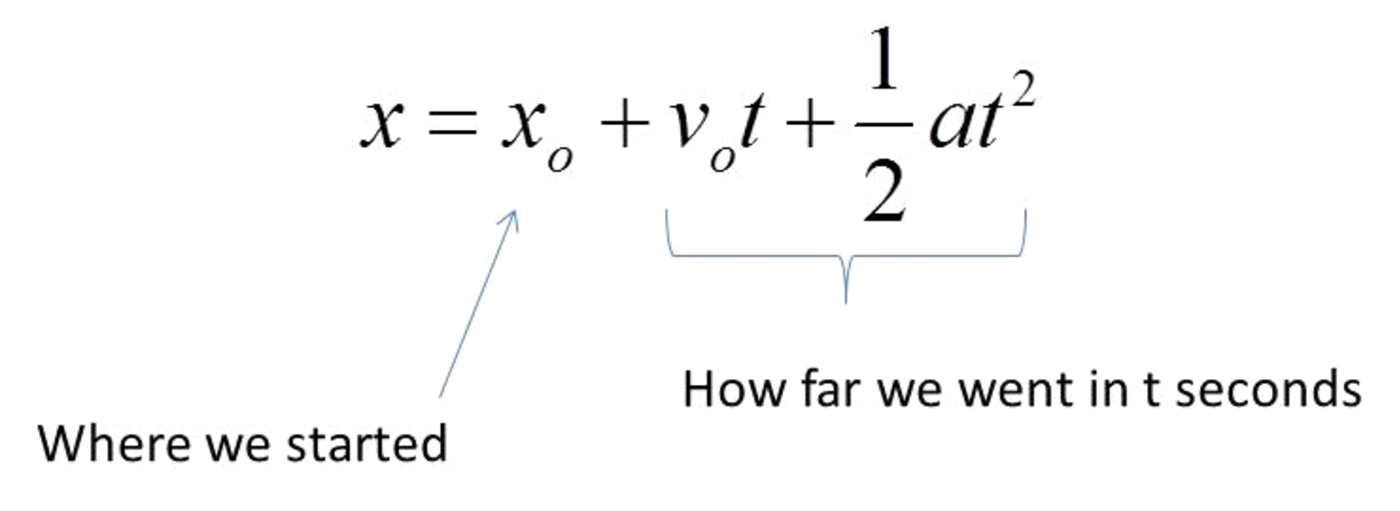
\includegraphics[width=0.8\textwidth]{Lab7_figs/kinematicsAnnotated.png} \end{center}
If the ball were going at constant speed, the additional distance would be
just $v_{o}t$. This comes from speed being distance over time.
\begin{align*}
v  & =\frac{d}{t}\\
d  & =vt
\end{align*}
But our ball is accelerating, so we have to add in a little more distance
because our speed is changing. That is what $\frac{1}{2}at^{2}$ does. 


Since the position is a function of $t^{2},$ we know that the position vs.
time graph for our ball will be a parabola.

 
\begin{center}
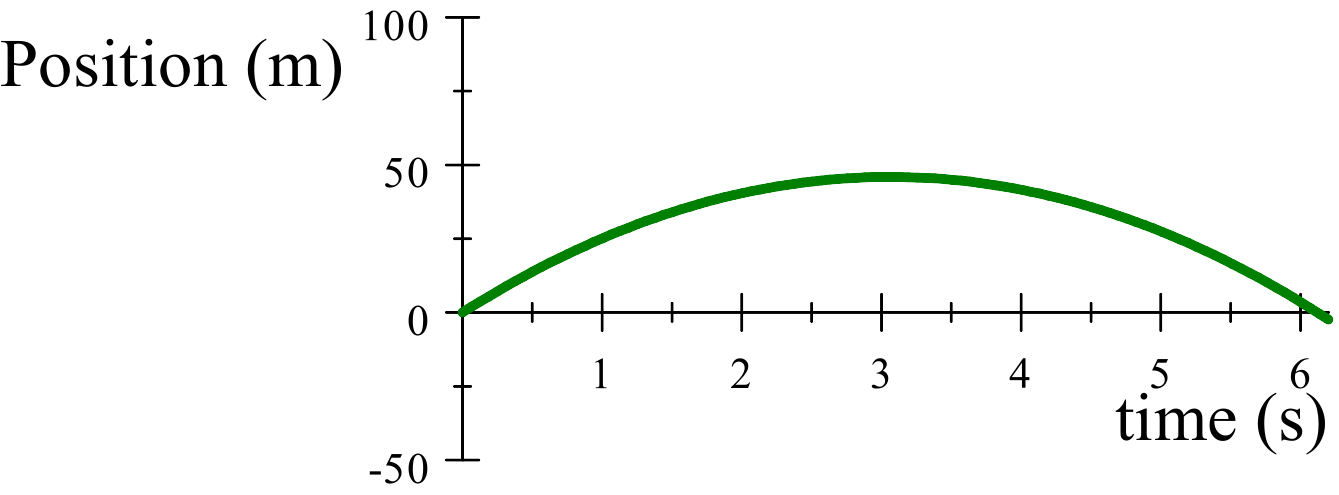
\includegraphics[width=0.8\textwidth]{Lab7_figs/PvTSimple.png}
\end{center}
The second and third equations from our kinematic set give the speed of the
object. The second is the speed as a function of time. Since for this first
problem in programming we will only allow one dimensional motion (at first) we
could say this is the velocity of the object and allow negative values to mean
going the opposite way of positive values. Because the ball is accelerating,
the speed will change. We can see that the velocity changes linearly with
time. Think of a straight line
\[
y=mx+b
\]
our velocity equation is
\[
v=at+v_{o}
\]
on a velocity vs. time graph, this has the form of a straight line. So the
velocity vs. time graph will be a straight line. 
\begin{center}
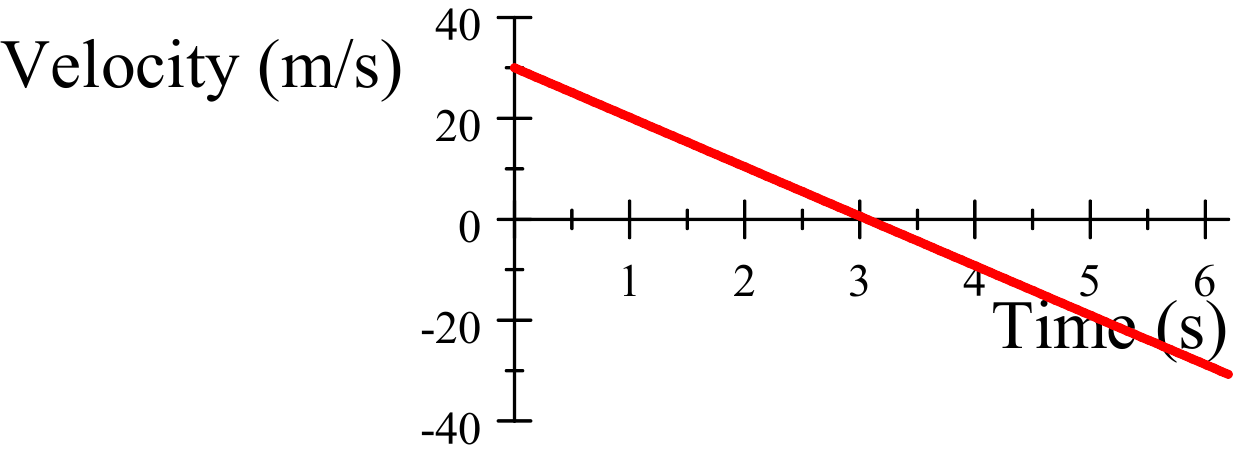
\includegraphics[width=0.8\textwidth]{Lab7_figs/VvTSimple.png}
\end{center}

\subsection{Changing Acceleration}
The kinematic equations only work when acceleration is constant. You should have learned in your physics class that you can get around this limitation by using the ending of one acceleration region as a starting point for the next. For example, imagine we have an acceleration that starts at $ 3 m/s^2$, but once a second goes down by one until it hits zero, like so:
\begin{center}
\begin{tblr}{colspec={c|c}}
t (s)& a (m/s$^2$)\\
\hline
0 & 3\\
1& 2 \\
2& 1\\
3 & 0


\end{tblr}
\end{center}

Since the acceleration is changing, we can't connect the beginning to the end with just one set of kinematic equations. However, if we knew that our initial velocity and position were both zero, we can find where we are and how fast we are going at one second:
\[ x_1 = x_0 + v_0t+\frac{1}{2}at^2 = 0 +0*1 + \frac{1}{2}*3*(1)^2 = 1.5\]
\[ v_1 = v_0 + at = 0+ 3*1 = 3\]

And then use that information to find out where we are and how fast we are going at 2 seconds:
\[ x_2 = x_1 + v_1t+\frac{1}{2}at^2 = 1.5 +3*1 + \frac{1}{2}*2*(1)^2 = 5.5\]
\[ v_2 = v_1 + at = 3+ 2*1 = 5\]

and so on until we fill out the table:
\begin{center}
\begin{tblr}{colspec={c|ccc}}
t (s)& a (m/s$^2$) & v (m/s) & x (m)\\
\hline
0 & 3 & 0 &0\\
1& 2  & 3&1.5\\
2& 1 & 5&5.5\\
3 & 0 &5 &10.5


\end{tblr}
\end{center}







\section{Euler's Method}


Euler's method works under this same principle (starting/ending new sets of kinematic equations), but it uses
an idea from calculus\footnote{Not to worry if you are concurrently taking
calculus. We will use very little calculus in this reading, so little that you
probably won't notice it.} that we can take an infinitesimally small amount of
time for our experiment. We will call this very small amount of time a
\textquotedblleft time step\textquotedblright\ and label it $\Delta t.$ Over
this time interval, the acceleration will be very close to constant, which lets us use kinematics. Our velocity equation looks the same:
\[v_f = v_i + a\Delta t \]
but our position equation will change a little bit. If $\Delta t$ is small, $\Delta t^2$ will be very very small, so the position question becomes:
\[
x_{f}=x_i+v_it+\frac{1}{2}at^2 \approx x_{i}+v_{i}\Delta t 
\]
since $\frac{1}{2}a\Delta t^2 \approx 0$\footnote{If acceleration is large enough that $\Delta t^2$ doesn't make this term almost zero, you need to pick a smaller $\Delta t$}.  In the limit as $\Delta t\rightarrow0$ our
equation will be exact.

Euler's method lets us calculate motion even when acceleration changes by following these basic steps:
\begin{itemize}
\item set up initial conditions (v,x)
\item Repeated section:
\begin{itemize}
\item Calculate my acceleration for my current position and velocity (for example: include a drag force that depends on how fast you are going)
\item Use the position equation and current velocity to find my next position
\item Use the velocity equation and current acceleration to find my next velocity

\end{itemize}

\end{itemize}


\subsection{Euler and Simple Systems with Not-So-Simple Dynamics.}

As an example, suppose we throw a ball, but we have air resistance. Your PH121 class only has
you throw balls in a vacuum--something that is only fun if you have a space
suit. Real balls have air resistance. To model air resistance is really a
PH123 problem. So I will just give you a formula for the force due to air
resistance here. There is a resistive force
\[
F_{R}=\frac{1}{2}D\rho Av^{2}
\]
that depends on the cross-sectional area of the ball, $A,$ the density of the
air, $\rho,$ the speed of the ball, $v,$ and the ball's drag coefficient, $D,$
that contains the effects like surface roughness and shape of the ball. So we
have two forces working on the ball now, the force due to gravity, and the
resistive force. If we throw the ball straight up, then we only have forces in
one dimension. We can use our Newton's second law method to find the acceleration! 
\[
\Sigma F_{x}=ma=-F_{g}+F_{R}
\]
so \[
a=\frac{-F_{g}+F_{R}}{m}
\]
or \begin{align*}
a  & =\frac{-mg+\frac{1}{2}D\rho Av^{2}}{m}\\
& =-g+\frac{D\rho Av^{2}}{2m} \end{align*}


Notice that this acceleration changes when $v$ changes. And we know that $v$
does change as the ball goes up. We can't use the kinematic equations at all
with a changing acceleration. But we can use our Euler method. \begin{align*}
x(t+\Delta t)  & =x(t)+v(t)\Delta t\\
v(t+\Delta t)  & =v(t)+a\left(  t\right)  \Delta t
\end{align*}
or \begin{align*}
x_{n+1}  & =x_{n}+v_{n}\Delta t\\
v_{n+1}  & =v_{n}+a_{n}\Delta t
\end{align*}
The only difference is that now our acceleration is not $-g,$ but
$a=-g+\frac{D\rho Av^{2}}{2m}.$ So instead of\footnote{The $x_{n+1}$ and $x_{n}$ is a standard notation to mean the next $x$ we find ($x_{n+1}$) compared to our current $x$ ($x_n$, the $x$ for right now). There are other algorithms that involve more points that might reference the previous ($x_{n-1}$) point we calculated, for example.}.
\begin{align*}
x_{n+1}  & =x_{n}+v_{n}\Delta t\\
v_{n+1}  & =v_{n}-g\Delta t
\end{align*}
we will have \begin{align*}
x_{n+1}  & =x_{n}+v_{n}\Delta t\\
v_{n+1}  & =v_{n}+\left(  -g+\frac{D\rho A\left(  v(t)\right)  ^{2}} {2m}\right)  \Delta t
\end{align*}


The rest of the method stays the same. In fact, to change physical systems we
usually only need to change the acceleration function. This implies that we
could build a general Euler solver, and then just modify the acceleration
part. That is such a good idea that there are standard notations for this.


\section{Implementation}

You are probably wondering how you would actually make a computer do all of
this calculation. In this section let's consider how to write an Euler method
code for our lab, then I will comment on versions to use in further studies
(later in your career). You don't need to read this section before class. What
follows is a tutorial that will guide you step-by-step through the first part
of the lab. But if you want to, read on just to get a feel for what we will do.



\subsection{The Program}
This program uses Euler's method to model an object falling straight down, with no air resistance.  Try to read through it and understand what it is telling the computer to do.  I will break it down piece by piece in the next section.
\begin{lstlisting}
"""
One Dimensional free-fall Euler Code

PH150
Brother Zachreson


This code will calculate the exact solution for a ball in free fall
having been shot straight up using Euler's method.

"""
#Import numerical and plotting packages
import numpy as np
import matplotlib.pyplot as plt


#Initial conditions and physical setup constants
v0=30.0 #Initial velocity in m/s
x0=70 #Initial Postion in m

#Set up the time steps and number of calculations
delta_t = 0.01 #Time step in seconds
t0=0 #Start time in seconds
t_max = 7.0 #Final time

#Calculate the number of timesteps we need to make
N=(t_max-t0)/delta_t

#Make sure N is an integer
N=int(N)


#Make lists to hold our positions, velocities, and times
x=[x0]
v=[v0]
t=[t0]

#Now perform an Euler's method calculation.
for i in range(N):
    #Find the current acceleration
    a=-9.8
    
    #Find the next velocity
    v.append(v[i]+a*delta_t)    
    
    
    #Find the next position
    x.append(x[i]+v[i]*delta_t)
    
    #increment our time
    t.append(t[i]+delta_t)

#End of Euler loop =========================================
#Plot the results
plt.plot(t,x,linewidth=2,color='red')
plt.xlabel('time (s)')
plt.ylabel('Position (m)')
plt.title('Position vs. time for a ball in free fall')
\end{lstlisting}


\subsection{The Program - Broken down}
This section will break the program down piece by piece. Here's the first section:
\begin{lstlisting}
"""
One Dimensional free-fall Euler Code

PH150
Brother Zachreson


This code will calculate the exact solution for a ball in free fall
having been shot straight up using Euler's method.

"""
#Import numerical and plotting packages
import numpy as np
import matplotlib.pyplot as plt
\end{lstlisting}

Everything inside the triple quotes |"""| counts as one long comment.  If you ever need to add comments that will take more than one line, you can start and end it with |"""|.  It's a great way to leave yourself notes about what each program does.
Below the introductory comment, I import Numpy and Matplotlib since I know that I'll be doing number crunching and plotting later on.

This next part sets up all of our constants and inputs.  It's a good idea to put it at the beginning of the program so that they are easy to change.
\begin{lstlisting}
#Initial conditions and physical setup constants
v0=30.0 #Initial velocity in m/s
x0=70 #Initial Postion in m

#Set up the time steps and number of calculations
delta_t = 0.01 #Time step in seconds
t0=0 #Start time in seconds
t_max = 7.0 #Final time

\end{lstlisting}

The part with |x0| and |v0| is where I set the starting position and velocity.  |delta_t| is how far forward in time we will go in each calculation.  Remember, Euler's method works by assuming that acceleration is roughly constant over short time intervals.  |delta_t| sets that time interval.

Once we know our initial values, we need to tell the computer how many calculations to do.  Here's the piece of code that does that:

\begin{lstlisting}
#Calculate the number of timesteps we need to make
N=(t_max-t0)/delta_t

#Make sure N is an integer
N=int(N)
\end{lstlisting}

The above code calculates the number of timesteps needed, then saves it in the variable |N|. 

Python keeps two types of numbers: ``Floats" - numbers with decimal points and ``Integers" - whole numbers. For example: 2.0 is a float, 2 is an integer.  Even though they have the same value, Python sees them as different things.
You can only get an item from a list using an integer.
|myList[2]| works, but |myList[2.0]| won't.  The command |N=int(N)| takes whatever number |N| is and converts it to an integer.  The |int| command truncates instead of rounding, so |int(2.9)| becomes |2|, not |3|.

\begin{lstlisting}
#Make lists to hold our positions, velocities, and times
x=[x0]
v=[v0]
t=[t0]

\end{lstlisting}
Notice that all three of these are in square brackets, but there aren't any on on the variables I set above (look back to where I set |x0|).  
Putting square brackets around something tells Python that it is a list.  Since we?re going to be adding more x,v, and t values, we need to warn Python that these are going to be lists.
Having the square brackets is essential on these. Whereas, |x0| is just a single value and will always be a single value, so it didn?t need square brackets.

This next section of code is what we call a loop:
\begin{lstlisting}
#Now perform an Euler's method calculation.
for i in range(N):
    #Find the current acceleration
    a=-9.8
    
    #Find the next velocity
    v.append(v[i]+a*delta_t)    
    
    
    #Find the next position
    x.append(x[i]+v[i]*delta_t)
    
    #increment our time
    t.append(t[i]+delta_t)

#End of Euler loop =========================================


\end{lstlisting}

\subsubsection{Breaking down the for loop}
For most of you, a loop will be a new idea. Loops are very helpful when you need to tell a computer to do something over and over again.  Here's the general structure:
\begin{lstlisting}
for <Thing that Changes>:
     Stuff the computer does to/with the thing that changes

Not part of the loop
\end{lstlisting}

Let's start by looking at the |Thing that Changes|.   As an example, here is a shopping list: bananas, apples, bread, milk.  If I wrote this program:
\begin{lstlisting}
shopping_list = ['bananas','apples','bread','milk']
for food in shopping_list:
    print(food)

print(shopping_list)
\end{lstlisting}
When I run this program, I first load my shopping list.  The |for food in shopping_list| tells Python to look at each thing in my list one by one, and call it |food|.  Therefore, this program would first print bananas, then when it sees that |print(shopping_list)| isn't indented, it knows to go back to the |for| line, but changes food to the next thing on the list: apples.  So, after printing bananas, then apples, it would print bread, then milk.  Since the list ends at milk, the computer would then know to continue on and print the whole shopping list at once. (Thanks to the |print(shopping_list)| command)

Now let's look at our |for| statement: |i in range(N)|.  The |range(N)| command makes a list of integers from zero to |N-1|.  If |N| was five, |range(N)| would be |[0,1,2,3,4]|.  Therefore, the first time we go through the for loop |i=0|, the second time |i=1|, and so on until we reach |N-1|.

Now let's look at the guts of the loop:
\begin{lstlisting}
    #Find the current acceleration
    a=-9.8
    
    #Find the next velocity
    v.append(v[i]+a*delta_t)    
    
    
    #Find the next position
    x.append(x[i]+v[i]*delta_t)
    
    #increment our time
    t.append(t[i]+delta_t)
\end{lstlisting}

This is where we actually implement Euler's method.  First we find the acceleration. (-9.8 in this case) Then, we have this command:
\begin{lstlisting}
v.append(v[i]+a*delta_t)
\end{lstlisting}
The |append| command takes whatever is in the parenthesis and adds it to the bottom of of whichever list is before the |.| . In this case, |v.append(v[i]+a*delta_t)| just adds |v[i]+a*delta_t| to the bottom of the |v| list.  
  
We know from kinematics that $v_f=v_i+a\Delta t$, so the program just uses |v[i]| as $v_i$, to calculate our ``final" velocity.  Each time the computer goes through the loop, it will use a different value for |i|, and therefore a different value for |v[i]|.  
If we start with |v=[0]|, the first time the computer gets to the loop, it will set |i=0|.  When it gets the the velocity line, it will go look up |v[0]|, which is just the first thing in |v|, or in our case, 0.  If |delta_t| is 0.1, then |v[0]+a*delta_t=0-9.8*.1=-.98|.  |v.append(-0.98)| would make our |v=[0,-0.98]|.  The second time through the loop, |i=1|, so |v[1]=-0.98|, since |v[1]| will give us the second thing in |v|.  Therefore |v[1]+a*delta_t=-.98-9.8*0.1=-1.96|, and with the append, our velocity list becomes |v=[0,-0.98,-1.96]|.  And the computer will continue repeating this process until we reach |i=N-1|.

We can also use our velocity to calculate our position.  We know from kinematics that $x_f=x_i+v_i\Delta t+\frac{1}{2}a\Delta t^2$.  In order for Euler's method to work, $\frac{1}{2}a\Delta t^2$ must be very small, so we ignore it.

Once the loop is finished, the program just builds a plot of the data:
\begin{lstlisting}
#Plot the results
plt.plot(t,x,linewidth=2,color='red')
plt.xlabel('time (s)')
plt.ylabel('Position (m)')
plt.title('Position vs. time for a ball in free fall')
\end{lstlisting}

\end{document}






\end{document}
